\section{Appendix}
\label{sec:appx}
\subsection{Cost estimates}

The cost estimates for drilling pipes downstream of the Hall A beam dump are based on a budgetary bid for a single 16" pipe at location C indicated in 
Fig.\,\ref{fig:ds-area}. A cross section of the pipe (or ``well") is shown in Fig.\,\ref{fig:Well_Section_Bid}. 
The budgetary quote was adjusted by Suresh Chandra (JLab Facilities) to account for additional effort/work needed to complete the 
project. The resulting cost estimate is shown in Fig.\,\ref{fig:Preliminary_Cost_Estimate_16_Inch_pipe-Rev1}. The following
items were included in the cost:
\begin{itemize}
\item concrete slab on grade as a base for experimental test
\item ground exploration in advance of drilling
\item air blower to keep the well dry during test
\item drilling of the hole proper; installing a pipe suitable for use as a guide for the detector apparatus
\item backfill and compaction
\item generator (on loan from facilities) to provide temporary power for one-week test (3KVA).
\end{itemize}

Based on the budgetary bid, two cost estimates were made for 10" pipes based on previous experience with such similar projects. The estimates are shown in 
Figs.\ref{fig:Preliminary_Cost_Estimate_10_Inch_pipe} and \ref{fig:Preliminary_Cost_Estimate_for_two_10_Inch_pipes} at locations B and C of  Fig.\,\ref{fig:ds-area}.
Given that the muon rate changes considerably with
distance to the dump, we believe that two pipes are necessary to reliably understand the rate measurements. The estimated cost to drill two 10" pipes is \$40k. 
The typical time schedule for completing the project would be 8 weeks to prepare the contract, 6 weeks to award, and 6 weeks to complete the work, i.e. five months
total.

\begin{figure}[thp] 
\center
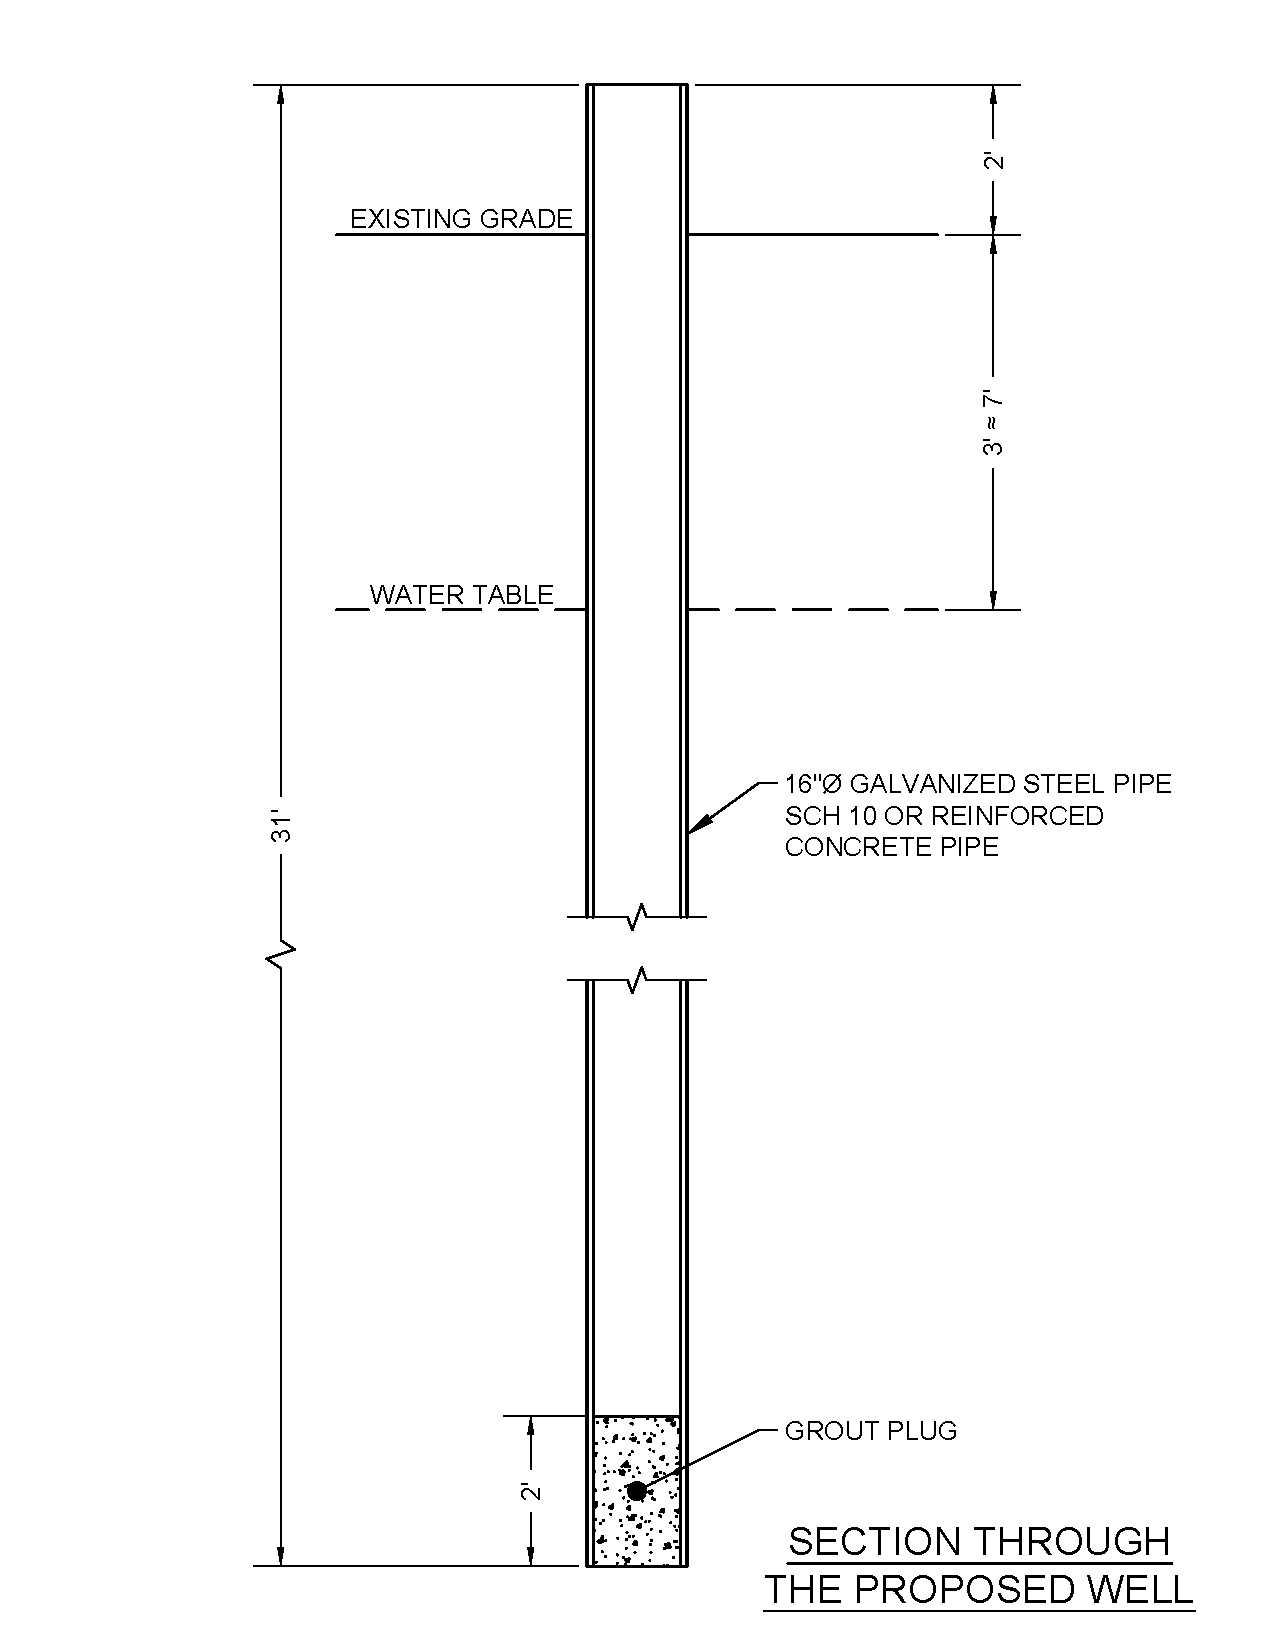
\includegraphics[width=8cm,clip=true]{figs/Well_Section_Bid.pdf}
\caption{Preliminary cost estimate for a single 16" pipe.}
\label{fig:Well_Section_Bid}
\end{figure}

\begin{figure}[thp] 
\center
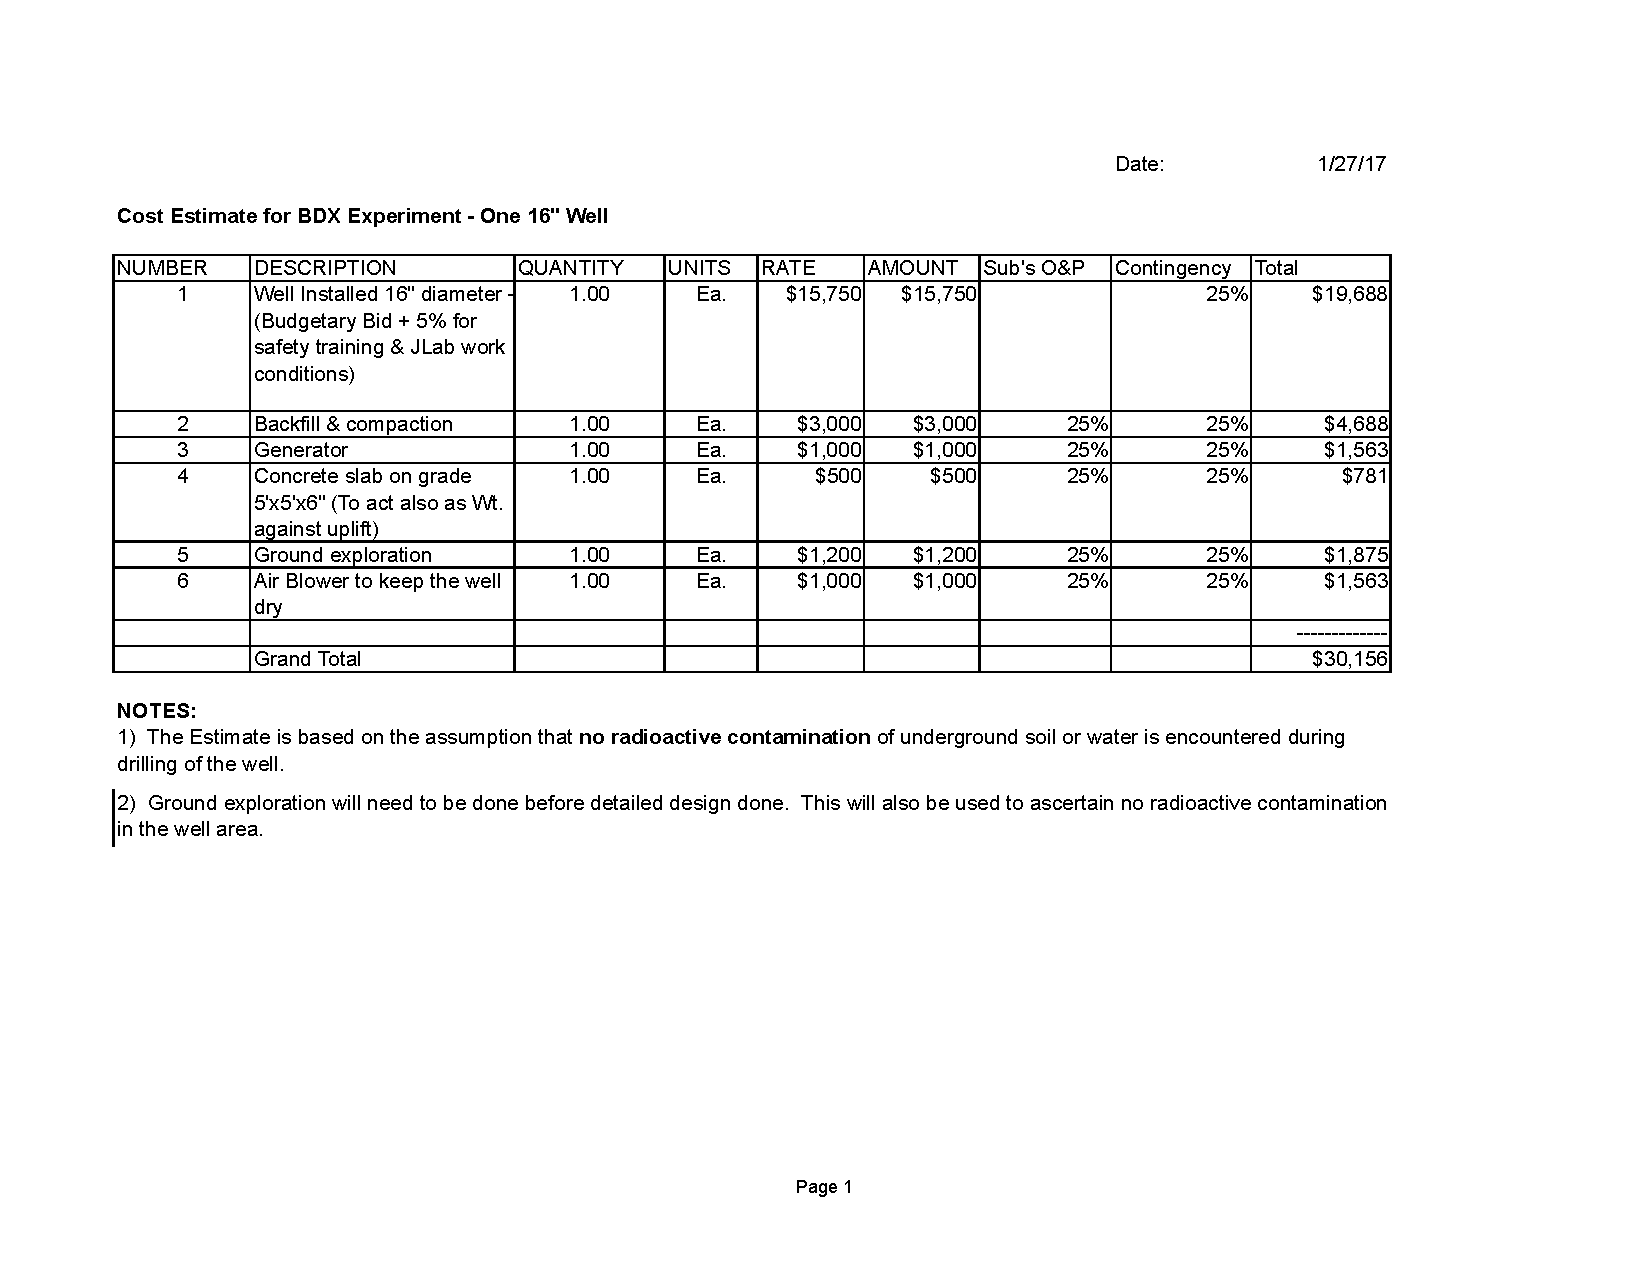
\includegraphics[width=17cm,clip=true]{figs/Preliminary_Cost_Estimate_16_Inch_pipe-Rev1.pdf}
\caption{Preliminary cost estimate for a single 16" pipe.}
\label{fig:Preliminary_Cost_Estimate_16_Inch_pipe-Rev1}
\end{figure}

\begin{figure}[thp] 
\center
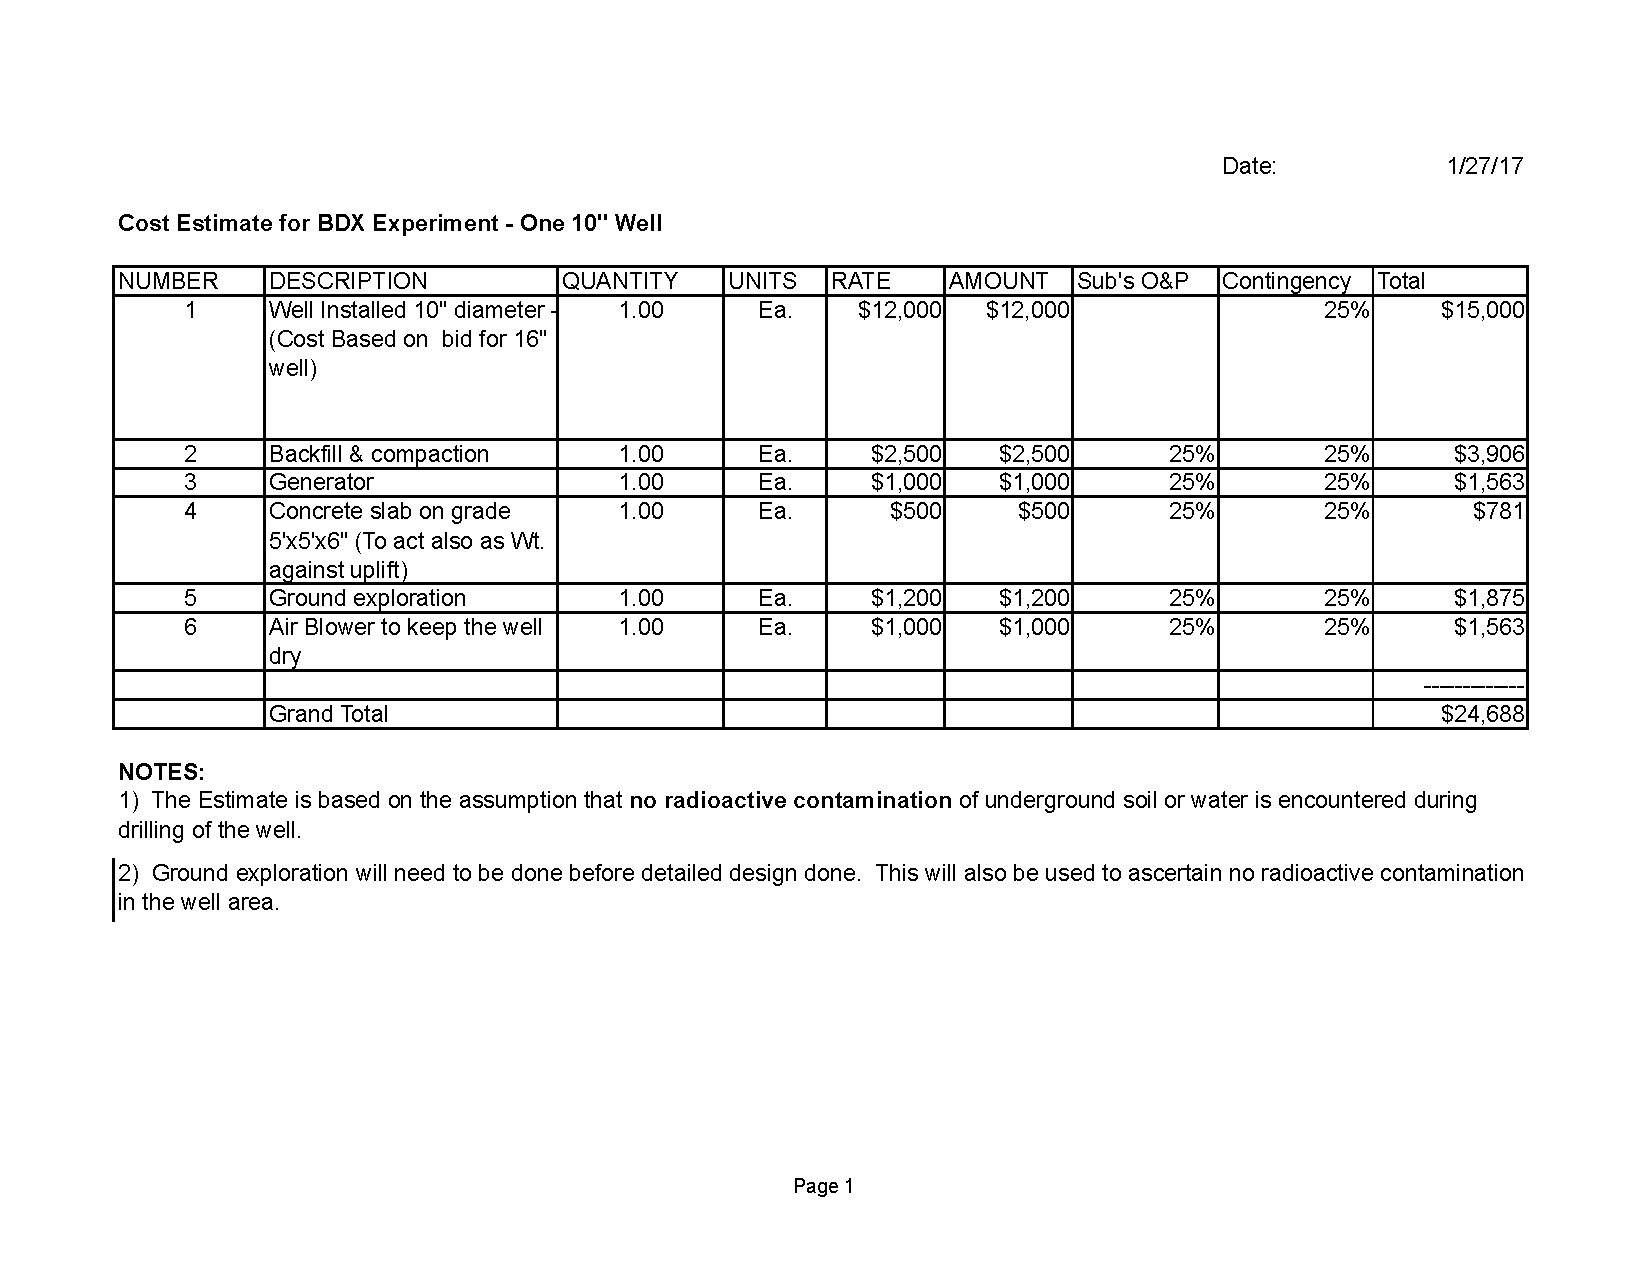
\includegraphics[width=17cm,clip=true]{figs/Preliminary_Cost_Estimate_10_Inch_pipe.pdf}
\caption{Preliminary cost estimate for a single 10" pipe.}
\label{fig:Preliminary_Cost_Estimate_10_Inch_pipe}
\end{figure}

\begin{figure}[thp] 
\center
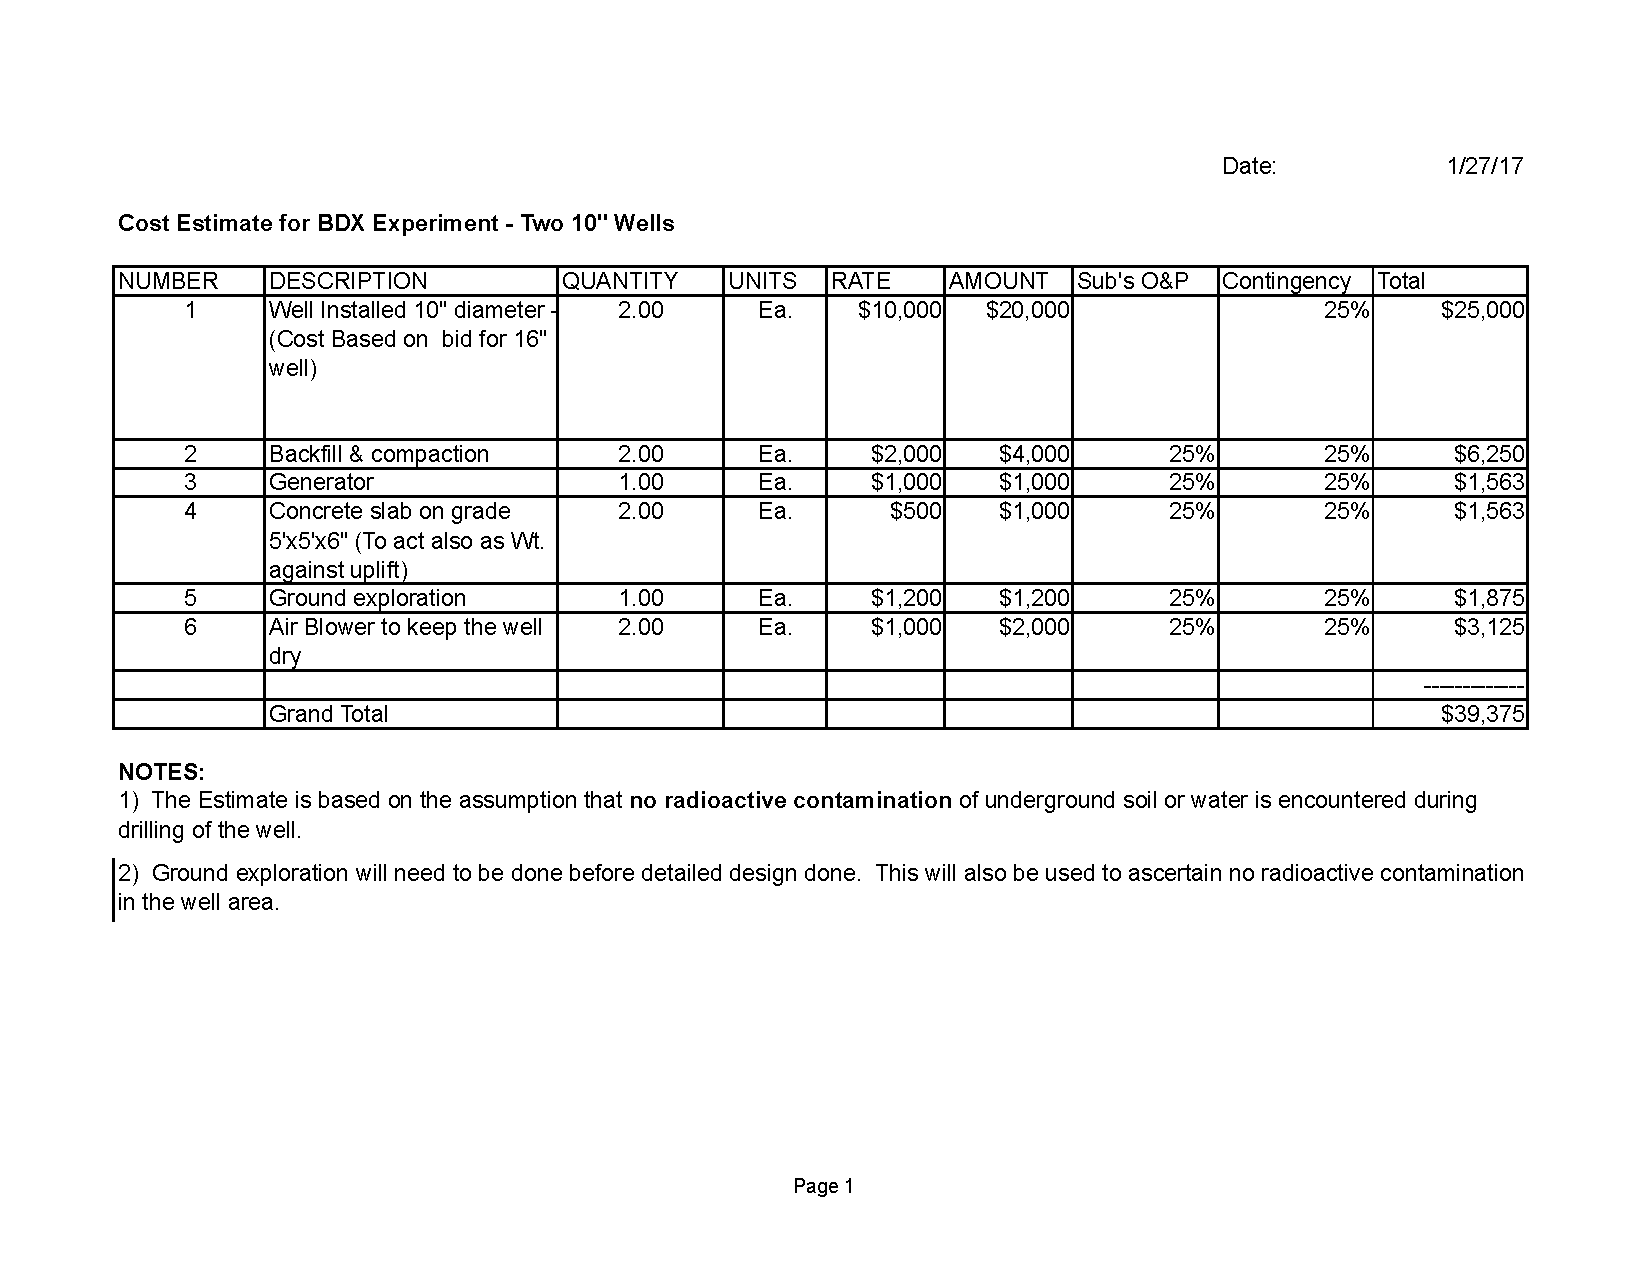
\includegraphics[width=17cm,clip=true]{figs/Preliminary_Cost_Estimate_for_two_10_Inch_pipes.pdf}
\caption{Preliminary cost estimate for two 10" pipes.}
\label{fig:Preliminary_Cost_Estimate_for_two_10_Inch_pipes}
\end{figure}


\subsection{Work- \& time-plan}
The two wells  will be drilled in locations {\bf B} and {\bf C} in the area downstream of Hall-A beam-dump as shown in Fig~\ref{fig:ds-area} inserting a 10" pipe as described in the previous Section. The test would requires to run during the day, approximately for 4 calendar  days (assuming a 50$\%$ efficiency of CEBAF to deliver 10 $\mu$A,  11 GeV electron beam\footnote{As already noticed, this measurement is possible for beam currents ranging from 1 to 100  $\mu$A.}.)
The detector will be lowered in the pipe and positioned at different depth tacking  data in each position. Table~\ref{tab:test} shows the expected CsI(Tl) rates and collected statistics.\
If possible  we would like to a do beam current scan to check the expect count rate scaling.
The only relevant information from the accelerator will be the beam-on status 
\begin{table}[htp]
\caption{Proposed test configuration}
\begin{center}
\begin{tabular}{|c|c|c|c|c|}
\hline\hline
\multicolumn{5}{r}{Preparation  $\sim$ 3h } \\
\hline
Position  &Depth  (cm)& Rate$_{Crystal} (kHz)$  &Run time (mn) & N$_{Evnt}$ collected (M)  \\
\hline\hline
 {\bf B} & 0 &  20 & 10 & 6\\
 \hline
 {\bf B}  & 40 &  10 & 20 & 6 \\
 \hline
 {\bf B}  & 80 &  4 & 40 & 5\\
 \hline
\multicolumn{5}{|r|}{Total time    $\sim$ 2h }\\
 \hline\hline
\multicolumn{5}{r}{Configuration change  $\sim$ 3h } \\
 \hline\hline
 {\bf C} & 0 &  2.8 & 30 & 5\\
 \hline
 {\bf C}  & 40 &  1.4 & 60 & 5 \\
 \hline
 {\bf C}  & 80 &  0.6 & 120 &4.5\\
 \hline
\multicolumn{5}{|r|}{Total time    $\sim$ 4h }\\
 \hline\hline
\end{tabular}
\end{center}
\label{tab:test}
\end{table}

